%%%%%%%%%%%%%%%%%%%%%%%%%%%%%%%%%%%%%%%%%%%%%%%%%%%%%%
% A Beamer template for Ritsumeikan University       %
% Author: Ming-Hao Xu (Xu Minghao)                   %
% Date:   April 2022.                                %
% LPPL Licensed.                                     %
%%%%%%%%%%%%%%%%%%%%%%%%%%%%%%%%%%%%%%%%%%%%%%%%%%%%%%

\documentclass{beamer}
\usepackage{hyperref}

\usepackage[UTF8]{ctex}
\usepackage[T1]{fontenc}

% other packages
\usepackage{latexsym,amsmath,xcolor,multicol,booktabs,calligra}
\usepackage{graphicx,pstricks,listings,stackengine}
\usefonttheme[onlymath]{serif}

% dummy text; remove it when working on this template
\usepackage{lipsum}

\author{Ebola}
\title{计算几何}
\institute{
    Institute of Mathematics, \\
    Zhejiang University.
}
\date{Jan, 2024}
\usepackage{Ritsumeikan}

% defs
\def\cmd#1{\texttt{\color{red}\footnotesize $\backslash$#1}}
\def\env#1{\texttt{\color{blue}\footnotesize #1}}
\definecolor{deepblue}{rgb}{0,0,0.5}
\definecolor{deepred}{rgb}{0.6,0,0}
\definecolor{deepgreen}{rgb}{0,0.5,0}
\definecolor{halfgray}{gray}{0.55}

\lstset{
    basicstyle=\ttfamily\tiny,
    keywordstyle=\bfseries\color{deepblue},
    emphstyle=\ttfamily\color{deepred},    % Custom highlighting style
    stringstyle=\color{deepgreen},
    numbers=left,
    numberstyle=\small\color{halfgray},
    rulesepcolor=\color{red!20!green!20!blue!20},
    frame=shadowbox,
}


\begin{document}

\begin{frame}
    \titlepage
\end{frame}

\begin{frame}
    \tableofcontents[sectionstyle=show,subsectionstyle=show/shaded/hide,subsubsectionstyle=show/shaded/hide]
\end{frame}

\section{二维几何基础}

\begin{frame}[fragile]{点与向量}
    二维平面上的任何一个点,可以用坐标 $(x,y)$ 表示。
    \vspace{1em}

    \pause
    向量是一个“具有方向和长度的箭头”,它不规定起点和终点。
    二维平面上的任何一个向量,也可以用坐标 $(x,y)$ 表示。
    \vspace{1em}

    \pause
    计算机存储点与向量没有区别,所以我们都可以用下面的结构体来存储。
\begin{lstlisting}[language=c++]
    struct Point{
        double x,y;
        Point(double x=0, double y=0): x(x), y(y) {}
    };
    #define Vector Point
    // 在计算机里,Vector 就是 Point,但为了从逻辑上区分,我们赋予它们不同的名字
\end{lstlisting}
\end{frame}


\begin{frame}[fragile]{浮点数比大小}
    \small
    浮点数是有限精度的,在运算过程中,难免会产生误差,
    相信大家深有被卡精度的体会。但是在计算几何中,我们
    经常需要判断浮点数的大小。\pause 这里我们引入如下的比较函数:
\begin{lstlisting}[language=c++]
    #define eps 1e-12
    int dcmp(double x)
    {
        if(fabs(x)<=eps) return 0;
        else if(x<0) return -1;
        else return 1;
    }
\end{lstlisting}
\end{frame}


\begin{frame}[fragile]{向量的基本运算}
    我们重载一些运算符来实现向量基本运算。
\begin{lstlisting}[language=c++]
    Vector operator + (Vector a, Vector b){return Vector(a.x+b.x, a.y+b.y);}
    Vector operator - (Vector a, Vector b){return Vector(a.x-b.x, a.y-b.y);}
    Vector operator - (Vector b){return Vector(-b.x, -b.y);}
    Vector operator * (Vector a, double x){return Vector(a.x*x, a.y*x);}
    Vector operator * (double x, Vector a){return Vector(a.x*x, a.y*x);}
    double Angle(Vector a){return atan2(a.y, a.x);}

    bool operator < (Point a, Point b){
        return a.x < b.x || (a.x == b.x && a.y < b.y);
    }
    bool operator == (Point a, Point b){
        return dcmp(a.x-b.x) == 0 && dcmp(a.y-b.y) == 0;
    }

    double Dot(Vector a, Vector b){return a.x*b.x + a.y*b.y;}
    double Length(Vector a){return sqrt(a.x*a.x + a.y*a.y);}
\end{lstlisting}
\end{frame}


\begin{frame}[fragile]{向量的叉乘}
    二维向量叉乘写作 $\mathbf{a}\times \mathbf{b}$,定义如下:
\begin{lstlisting}[language=c++]
    double Cross(Vector a,Vector b){return a.x*b.y - a.y*b.x;}
\end{lstlisting}

    \vspace{1em}\pause
    在几何中,叉乘是向量 $\mathbf{a}$ 与 $\mathbf{b}$ 构成的平行四边形的有向面积。
    如果 $\mathbf{b}$ 在 $\mathbf{a}$ 的\textbf{逆时针}方向,
    结果就是\textbf{正}的;否则就是负的。

    \begin{figure}
        \centering
        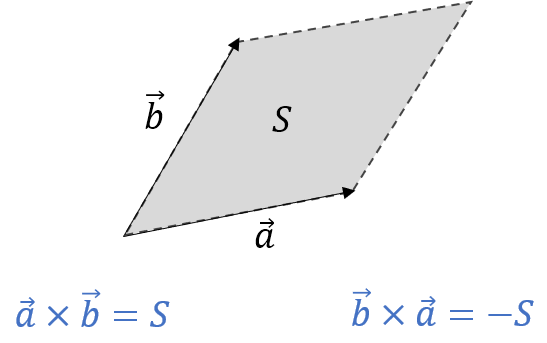
\includegraphics[width=0.4\textwidth]{pic/cross.png}
    \end{figure}
\end{frame}


\begin{frame}[fragile]{叉乘的应用:将凸多边形的顶点按逆时针排序}
    给定凸 $n$ 边形的所有顶点,请将它们按逆时针排序,起点随意。

    (提示:使用 \verb|sort| 函数,考虑如何定义 \verb|cmp|)

    \vspace{1em}\pause
    先随意固定一个起点 $P_0$,$P_i$ 排在 $P_j$ 前面,当且仅当
    \begin{equation*}
        \overrightarrow{P_0P_i} \times \overrightarrow{P_0P_j} > 0.
    \end{equation*}

    \begin{figure}
        \centering
        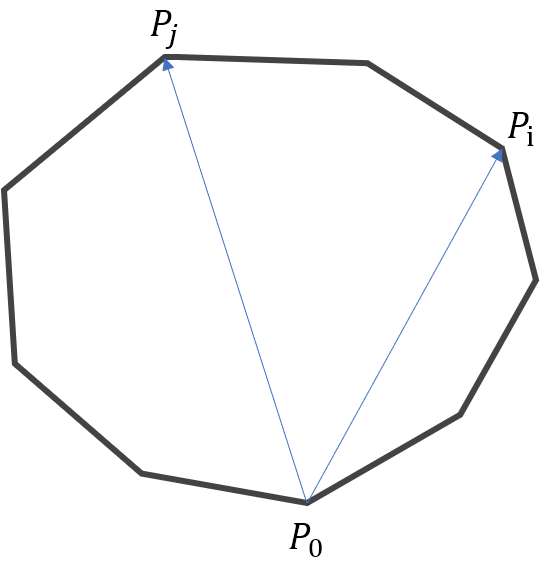
\includegraphics[width=0.4\textwidth]{pic/sort.png}
    \end{figure}
\end{frame}


\begin{frame}[fragile]{叉乘的应用:求凸多边形的面积}
    给定凸 $n$ 边形的所有顶点,它们已经按逆时针排好了序,求图形的面积。

    \vspace{1em}\pause
    \begin{figure}
        \centering
        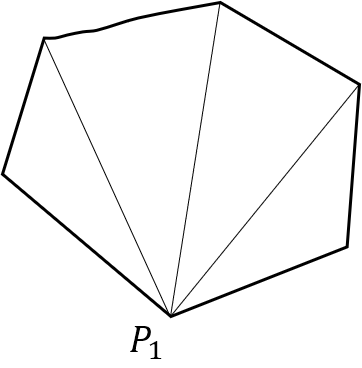
\includegraphics[width=0.3\textwidth]{pic/area.png}
    \end{figure}
    依次叉乘并累加即可。
\begin{lstlisting}[language=c++]
    double area = 0;
    for(int i = 2; i <= n-1; i++)
        area += 0.5 * cross(p[i]-p[1], p[i+1]-p[1]);
\end{lstlisting}
\end{frame}


\begin{frame}
    \begin{center}
        {\Huge\calligra Thank You}
    \end{center}
\end{frame}

\end{document}